\receita{Stir Fry de Frango\checkmark}{
\begin{itemize}
    \item 1 meio-peito de frango
    \item Verduras apropriadas (cenoura, brócolis, acelga)
    \item 1 dente de alho
    \item Molho shoyu
    \item Óleo para fritar
    \item Gengibre, bem pouco.
\end{itemize}
}{
\begin{enumerate}
    \item Cortar o frango em tirinhas
    \item Ralar 1 dente de alho inteiro.
    \item Colocar um pouco de óleo numa frigideira ou wok, e colocar o alho ralado e gengibre por alguns segundos.
    \item Colocar o frango quando a panela já estiver quente. Virar bastante para não deixar queimar.
    \begin{itemize}
        \item Se não estiver quente o suficiente, o frango irá perder água e vai ficar seco.
        \item Se tiver muito frango, fazer a fritura do mesmo em várias porções, de acordo com o tamanho da frigideira e da potência do fogo.
    \end{itemize}
    \item Quando dourado, retirar o frango e colocar armazenado em outro lugar.
    \item Fritar as verduras e legumes até ficarem cozidas.
    \begin{itemize}
        \item Colocar sempre os mais duros antes
        \item Caso tenha brócolis, branquear (ferver água, deixar 2-3 minutos, escorrer)
        \item Caso tenha acelga, coloque por último 
    \end{itemize}
    \item Voltar o frango, aquecer um pouco, colocar 1 colher de sopa de shoyu, mexer bem para incorporar. Vai ficar mais escuro do que aparenta no início. \begin{itemize} \item Se tiver macarrão, colocar o shoyu antes, incorporar, depois colocar o macarrão. \item Tomar cuidado com não deixar a tampa do shoyu sair e derramar demais. \end{itemize}
\end{enumerate}

\fotoreceita{0.7\textwidth}{./Fotos/Stir_Fry.png}
}

\receita{Bife com Curry\checkmark}{
    \begin{itemize}
    \item Carne
    \item Alho
    \item Cebola
    \item Óleo/manteiga
    \item Curry em pó
    \end{itemize}
}{
    \begin{enumerate}
    \item Cortar a carne em tiras
    \item Fritar cebola e alho bem picadinho, refogar com óleo ou manteiga, colocar a carne e refogar uns minutos.
    \begin{enumerate}
        \item Como vai usar curry, pode soltar água da carne. 
        \item Caso não solte a água, abaixa o fogo e coloca a tampa e espera um pouco. Caso não solte ainda, coloca meio copo de água quente.
    \end{enumerate}
    
    \item Aí põe algo como uma colher de sopa de curry e termina de refogar. Serve com arroz.
    \end{enumerate}
}

\receita{Arroz na panela de arroz\checkmark}{
\begin{itemize}
    \item Arroz. Geralmente, para 2, um copo é o suficiente.
    \item Alho. Para 2, meio alho está bom.
    \item Cebola. Para 2, meia cebola pequena está bom
    \item Óleo. Suficiente para cobrir o fundo da panela com um filmezinho.
    \item Água quente
\end{itemize}
}{
\begin{enumerate}
    \item Colocar a água para esquentar. %
    \begin{itemize} \item Opcional. Se colocar, (deve) diminuir o tempo de cozimento no final. \end{itemize}
    \item Colocar o alho e cebola finamente picados numa panela com óleo para dourar. \begin{itemize} \item Pode adicionar o alho depois para diminuir a chance de queimar ele.  \end{itemize}
    \item Colocar o arroz e fritar um pouquinho. Transferir tudo para a panela de arroz. Colocar a água na proporção de 2 copos de água para 1 copo de arroz (medida da panela).
\end{enumerate}
}

\receita{Pique Macho\checkmark}{
\begin{itemize}
    \item Batata para fritar
    \item Cebola roxa
    \item Tomate
    \item Pimentão (locoto)
    \item Salsicha
    \item Lombo
    \item Pimenta do reino
    \item Cominho
    \item Mostarda
    \item Shoyu (relativamente pouco, 2 colheres para 1kg de carne)
    \item Sal
    \item Óleo de girassol
    \item Ovos
    \item Maionese
    \item Ketchup
\end{itemize}
}{
\begin{enumerate}
    \item Fritar as batatas
    \item Fritar a carne, sem se preocupar em selar. Parte do sabor do prato vem do líquido soltado pela carne.
    \item Colocar o cominho, pimenta, mostarda, shoyu e sal com a carne ainda vermelha.
    \item Colocar os ovos para cozinhar em outra panela.
    \item Deixar a carne cozinhar.
    \item Colocar a salsicha e esperar 5 minutos, desligar o fogo.
    \item Colocar a carne sobre as batatas fritas.
    \item Colocar as cebolas que estavam no vinagre para perder o sabor forte, tomate, ovos cozidos, pimentões verdes, sobre o prato.
\end{enumerate}
}

\receita{Macarrão com manteiga, ovo e queijo\checkmark}{
\begin{itemize}
    \item Espaguete.
    \item Sal
    \item 3/4 copo de leite
    \item 1 ovo
    \item 2 colheres de manteiga
    \item 2/3 copo de parmesão ralado
    \item Pimenta a gosto
\end{itemize}
}{
\begin{enumerate}
    \item Cozinhar o macarrão numa panela. \begin{itemize}
        \item Colocar sal na água. Deixar ferver. Colocar macarrão.
    \end{itemize}
    \item Escorrer o macarrão ao ficar al dente.
    \item Devolver o macarrão na panela, abaixar a temperatura, colocar a mistura de leite, ovo e manteiga, e mexer até recobrir o macarrão. \begin{itemize}
        \item Quando eu fiz, deixei bastante tempo para garantir que o ovo estivesse cozido. Ele engrumou, mas a Karen gostou de qualquer forma.
    \end{itemize}
    \item Remover o calor. Colocar queijo e misturar. Se estiver pastoso demais, colocar mais lente.
\end{enumerate}
}

\receita{Caldo de frango\checkmark\label{rec:caldo_frango}}{
\begin{itemize}
    \item 3 dentes de alho
    \item 1 cebola pequena
    \item 2 coxas de frango, 2 sobrecoxas de frango, 2 meio-peitos
    \item Óleo
    \item Sal
\end{itemize}
}{
\begin{enumerate}
    \item Cortar bem pequeno o alho e a cebola. Colocar ambos para dourar um pouco de tempo. Colocar uma colher de chá de sal.
    \item Colocar o frango, sem tirar a pele ou qualquer outra coisa.
    \item Colocar a água. Cerca de 2 litros, ou até cobrir tudo. Deixar a panela no fogo alto até a água começar a ferver, depois colocar no fogo médio.
    \item Tempo total é de cerca de 1h depois de começar a ferver. Mexer no frango de vez em quando para ver a textura e possivelmente abrir os pedaços para ajudar a cozinhar.
    \begin{itemize}
        \item Dá para remover o peito antes dos outros porque deve cozinhar antes, e se ficar tempo demais fica duro.
    \end{itemize}
    \item Estará pronto quando notar que a carne está saindo dos ossos.
    \item Coar tudo por uma peneira. Reservar o frango para fazer uma torta ou alguma coisa assim. 
\end{enumerate}
}

\receita{Risoto de parmesão\checkmark}{
\begin{itemize}
    \item 2,5 copos de caldo de frango (vide receita \ref{rec:caldo_frango})
    \item 0,75 copos de água
    \item 2 colheres de sopa de manteiga
    \item 0,5 cebola grande, finamente cortada
    \item Sal, pimenta
    \item 0,5 dente de alho, cortado finamente
    \item 1 copo de arroz para risoto (arbório ou outro)
    \item 25-30g de parmesão ralado
    \item 1 colher de sopa de salsinha e cebolinha
    \item 0,5 colher de sopa de suco de limão
\end{itemize}
}{
\begin{enumerate}
    \item Ferver o caldo e a água em panela grande em fogo quente. Depois reduzir o calor para um fervor gentil.
    \item Derreter metade da manteiga numa panela\footnote{De preferência de ferro, mas pode ser alguma com uma massa térmica maior que uma panela comum} em calor médio. Colocar a cebola e 0,75 colher de sopa de sal. Ir mexendo por 5 a 7 minutos.
    \item Colocar o alho até ficar cheiroso, 30 segundos.
    \item Colocar o arroz e cozinhar, mexendo lentamente até os grãos ficarem translúcidos nas bordas, 3 minutos. 
    \begin{itemize}
        \item Cuidado com deixar o arroz queimar nesta etapa! Mexer bastante.
    \end{itemize}
    \item Colocar o caldo aquecido até cobrir o arroz. Reduzir o calor para médio-baixo. Ficar mexendo até absorver. Quando secar, adicionar mais caldo em parcelas bem pequenas. Sempre ficar mexendo para garantir que não vai queimar. Continuar até o arroz ficar cremoso e cozido, ou acabar o caldo. 16-19 minutos.
    \item Colocar o parmesão e mexer. Remover do calor, cobrir, e deixar parado por 5 minutos.
    \item Colocar o resto da manteiga, salsinha, cebolinha e limão.
    \begin{itemize}
        \item O limão não foi muito bem quisto pela Karen. Dá para colocar a salsinha e cebolinha, separar em duas metades, e em uma delas colocar 0,25 colher de sopa do suco de limão.
    \end{itemize}
\end{enumerate}

\fotoreceita{0.7\textwidth}{./Fotos/Risoto}
}

\receita{Conchiglioni de queijo\checkmark}{
\begin{itemize}
    \item Aproximadamente 50 Conchiglioni
    \item 1 cilindro de ricota fresca. Mais molinha é melhor (cerca de 200g?)
    \item 1 pote de creme de ricota.
    \item 100g de mussarella ralada
    \item 100g de provolone ralado
    \item 25g de parmesão ralado para recheio, um pouco para polvilhar em cima
    \item molho de tomate pronto. 1 saquinho para pouco molho, 2 para banhar bem.
    \item sal
    \item nozes picadas, aproximadamente 8
\end{itemize} }{
\begin{enumerate}
    \item Cozinhar os conchiglioni em água com sal até ficarem no ponto.
    \item Enquanto cozinha, misturar todos os queijos juntos, com as nozes. Provar se tem sal suficiente e colocar um queijo ou outro para atingir o sabor. Senão, colocar sal, mas por experiência, para meu gosto, isso não é necessário.
    \item Ao terminar, coar o macarrão, deixar esfriar um pouco. Começar a aquecer o forno a 200 $^\circ$C.
    \item Numa travessa grande, cobrir a base com molho de tomate, para evitar do macarrão queimar durante o assamento.
    \item Preencher generosamente os conchiglioni com o recheio. Colocar na travessa da maneira mais eficiente possível, porque 50 conchiglioni é bastante.
    \item Jogar molho por cima deles, tentando ser homogêneo, mas não é necessário. Após, salpicar parmesão a gosto.
    \item Colocar no forno por 15 minutos. Se tiver duas travessas, retirar a travessa de baixo, mais perto do fogo, antes, para que não queime. O interessante é derreter o recheio e aquecer tudo, pois a comida já está tecnicamente pronta para ser comida.
    \item Servir e comer imediatamente. O que sobrar pode ser resfriado ou congelado e posteriormente aquecido no micro ondas que não há perda de sabor.
\end{enumerate}
}

\receita{Frango tailandês com manjericão}{
\begin{itemize}
    \item 1 meio peito de frango cortado em pedaços \emph{bite-sized}
    \item 1 a 2 pimentas vermelhas, a critério pessoal
    \item 2 a 4 dentes de alho
    \item 1 ramo de manjericão
    \item 1 a 2 colheres de sopa de shoyu
    \item 1 colher de sopa de molho de ostra (opcional)
    \item 1 colher de chá de açúcar cristal.
\end{itemize}
}{
\begin{enumerate}
    \item Cortar o frango e reservar
    \item Macerar a pimenta e o alho juntos
    \item Separar as folhas do manjericão do caule
    \item Começar a aquecer o wok com óleo até ficar bem quente.
    \item Fritar o macerado de alho e pimneta por alguns segundos, mexendo sempre
    \item Acrescentar o frango e stir fry por 2 minutos. Não pode estar cru nem cozido demais.
    \item Acrescentar o molho de soja, de ostra, açúcar e mais stir fry por 15 segundos.
    \item Acrescentar o manjericão, misturar, e desligar o fogo imediatamente.
    \item Servir bem quente com arroz pré-preparado e guarnecer com ovo por cima
\end{enumerate}

\noindent \textbf{Acompanhamentos}
\begin{itemize}
    \item Arroz branco, tipo Jasmim ou japonês, e ovo frito.
\end{itemize}
}

\receita{Panqueca salgada}{
    \begin{itemize}
        \item 3 ovos
        \item 200 mL de leite integral
        \item 100 g de farinha de trigo
        \item 50 g de manteiga derretida
        \item sal
    \end{itemize}
}{
    \begin{itemize}
        \item Peneirar a farinha.
        \item Fazer um buraco no meio da farinha e colocar os ovos. Mexer com fouet.
        \item Colocar o leite aos poucos para não formar pelotas.
        \item Derreter a manteiga numa panela separada e incorporar na massa.
        \item Descansar a massa por pelo menos 1h, idealmente 5, na geladeira.
        \item Untar uma frigideira e fritar em camadas bem finas, em fogo médio/alto.
    \end{itemize}
}

\receita{Ovos diabólicos}{
    \begin{itemize}
        \item Ovos
        \item Creamcheese
        \item Pimenta vermelha
        \item Sal
        \item Mostarda
    \end{itemize}
}{
    \begin{enumerate}
        \item Cozinhar os ovos por 5 minutos, colocando-os em água gelada posteriormente para ajudar a soltar a casca.
        \item Cotar os ovos perpendicularmente para tirar as gemas.
        \item Misturar as gemas com creamcheese, pimenta vermelha, sal, mostarda.
        \item Quando a mistura estiver bem lisa, sem grumos, colocar num saquinho, cortar a ponta e preencher os espaços da gema na clara cozida.
    \end{enumerate}
}

\receita{Nhoque a bolonhesa\checkmark}{

\textsc{Nhoque}

\begin{itemize}
    \item 600g de batatas Asterix
    \item 1 ovo
    \item 2 xícaras de chá de parmesão ralado fino
    \item 1 colher de sopa de manteiga
    \item Pimenta síria a gosto
    \item 1 colher de sopa de farinha de trigo
    \item 1 fio de azeite e sal para a água do cozimento
\end{itemize}

\textsc{Molho bolonhesa\checkmark}

\begin{itemize}
    \item 1 colher de sopa de óleo ou azeite
    \item 1 cebola média picada
    \item 2 dentes de alho
    \item 1 kg de carne moída
    \item Orégano
    \item Pimenta do reino
    \item Colorau
    \item Sal
    \item 1 lata de extrato de tomate
    \item 1 sachê de molho de tomate
    \item 1 xícara de chá de água
\end{itemize}
}{

\textsc{Nhoque}

\begin{enumerate}
    \item Cozinhar as batatas, amassar ainda quente. (com casca?)
    \item Aguardar as batatas esfriarem. Adicionar os outros ingredientes até formar uma massa tipo pão leve. Se necessário, adicionar mais farinha (o que observar?)
    \item Ferver água com um fio de azeite.
    \item Fazer rolinhos e cortar a massa em tubos curtos. Colocar na água fervente.
    \item Quando a massa boiar, retirar da água.
\end{enumerate}

\textsc{Molho bolonhesa}
\begin{enumerate}
    \item Numa panela média, refogue a cebola e o alho no óleo ou no azeite até dourar.
    \item Em seguida adicione a carne moída e tempere com orégano, pimenta do reino, colorau, sal a gosto.
    \item Mexer para misturar bem e refogar por aproximadamente 10 minutos.
    \item Adicionar o extrato, molho e água.
    \item Misturar, tampar a panela e deixar cozinhar por mais 5 minutos.
    \item Desligar o fogo
\end{enumerate}

\begin{center}
    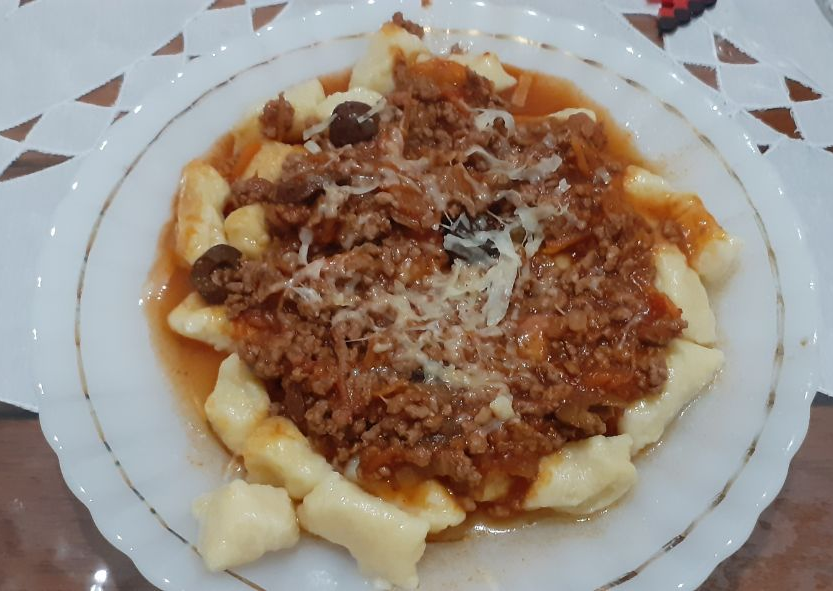
\includegraphics[width=0.7\textwidth]{Fotos/Nhoque.png}
\end{center}
}